\documentclass[
	12pt,
	openright,
	oneside,
	a4paper,
	english,
	brazilian,
	]{ufsj-abntex2}

\usepackage{cmap}
\usepackage{lmodern}
\usepackage[T1]{fontenc}
\usepackage[utf8]{inputenc}
\usepackage{lastpage}
\usepackage{indentfirst}
\usepackage{color}
\usepackage{graphicx}
\usepackage{multicol}
\usepackage{float}
\usepackage[table,xcdraw]{xcolor}
\usepackage{tikz}
\usetikzlibrary{positioning}

\providecommand{\htmladdnormallink}[2]{\href{#2}{#1}}

\usepackage[brazilian,hyperpageref]{backref}
\usepackage[alf]{abntex2cite}

\renewcommand{\backrefpagesname}{Citado na(s) página(s):~}
\renewcommand{\backref}{}
\renewcommand*{\backrefalt}[4]{
	\ifcase #1 %
		Nenhuma citação no texto.%
	\or
		Citado na página #2.%
	\else
		Citado #1 vezes nas páginas #2.%
	\fi}%

\titulo{Índice temporal informacional a partir de notícias corporativas: uma proposta para empresas brasileiras de saneamento}
\autor{Gabriel Felipe Souza Santos}
\local{São João del-Rei}
\data{\the\year}
\orientador{Michel Carlo Rodrigues Leles}
\instituicao{%
  Universidade Federal de São João del-Rei -- UFSJ
  \par
  Programa de Pós-Graduação em Ciência da Computação -- PPGCC
  \par
  Mestrado em Ciência da Computação}
\tipotrabalho{Dissertação (Mestrado)}
\preambulo{Dissertação apresentada como requisito para obtenção do título de mestre em Ciência da Computação no Programa de Pós-Graduação em Ciência da Computação da Universidade Federal de São João del-Rei.}

\definecolor{blue}{RGB}{41,5,195}

\makeatletter
\hypersetup{
		pdftitle={\@title},
		pdfauthor={\@author},
    	pdfsubject={\imprimirpreambulo},
	    pdfcreator={LaTeX with abnTeX2},
		pdfkeywords={sentimento, noticias, saneamento, indice temporal, NLP},
		colorlinks=true,
    	linkcolor=blue,
    	citecolor=blue,
    	filecolor=magenta,
		urlcolor=blue,
		bookmarksdepth=4
}
\makeatother

\setlength{\parindent}{1.3cm}
\setlength{\parskip}{0.2cm}

\makeindex

\begin{document}

\frenchspacing

\pretextual
\imprimircapa
\imprimirfolhaderosto*{Folha de rosto}
\begin{folhadeaprovacao}

  \begin{center}
    {\ABNTEXchapterfont\large\imprimirautor}

    \vspace*{\fill}\vspace*{\fill}
    {\ABNTEXchapterfont\bfseries\Large\imprimirtitulo}
    \vspace*{\fill}

    \hspace{.45\textwidth}
    \begin{minipage}{.5\textwidth}
        \imprimirpreambulo
    \end{minipage}%
    \vspace*{\fill}
   \end{center}

   Trabalho aprovado. \imprimirlocal, \today:

   \assinatura{\textbf{\imprimirorientador} \\ Orientador}
   \assinatura{\textbf{Membro da banca} \\ A definir}
   \assinatura{\textbf{Membro da banca} \\ A definir}

   \begin{center}
    \vspace*{0.5cm}
    {\large\imprimirlocal}
    \par
    {\large\imprimirdata}
    \vspace*{1cm}
  \end{center}

\end{folhadeaprovacao}

\begin{agradecimentos}
Este manuscrito registra a fundamentação inicial da pesquisa de mestrado junto ao PPGCC/UFSJ. Agradeço ao orientador Michel Carlo Rodrigues Leles pelo acompanhamento e à Universidade Federal de São João del-Rei pelas condições de trabalho.
\end{agradecimentos}

\begin{resumo}

Notícias financeiras em português carregam informação que o mercado pode precificar, mas transformar esse texto em uma série temporal reprodutível ainda é um problema aberto --- sobretudo em setores pouco cobertos pela literatura de processamento de linguagem natural. Esta dissertação fundamenta a proposta de um Índice Temporal Informacional (ITI) a partir de notícias corporativas de empresas brasileiras de saneamento de capital aberto, descreve o protocolo operacional já montado no laboratório e registra andamentos experimentais sem fechá-los como resultado. O ITI não replica um índice publicado: toma a cadeia metodológica ``texto agregado no tempo e validado externamente'', o escore de sentimento de domínio em português e a tradição de comparar medidas simples antes de construções mais elaboradas. A lacuna é a ausência de um microíndice empresa a empresa, baseado em notícias, para o saneamento --- setor marcado pelo Marco Legal e por eventos institucionais como a privatização da Sabesp. A avaliação de desempenho permanece em aberto, condicionada à qualidade do classificador no domínio.

\vspace{\onelineskip}

\noindent
\textbf{Palavras-chave}: sentimento de notícias; índice temporal; saneamento; processamento de linguagem natural; mercado brasileiro.
\end{resumo}

\begin{resumo}[Abstract]
\begin{otherlanguage*}{english}

Financial news in Portuguese can carry information that markets may price, yet turning that text into a reproducible time series remains an open problem --- especially in sectors that NLP research has barely covered. This dissertation motivates an Informational Temporal Index (ITI) built from corporate news about publicly listed Brazilian sanitation firms, describes the operational protocol already in place in the laboratory, and records preliminary experiments without treating them as final results. The ITI is not a copy of a published index: it borrows the methodological chain of aggregating text over time and validating it externally, a Portuguese domain sentiment score, and the habit of comparing simple baselines before a more elaborate construction. The gap is the lack of a firm-level, news-based index for sanitation --- a sector shaped by the Sanitation Legal Framework and institutional events such as Sabesp's privatization. Performance evaluation remains open, conditional on classifier quality in this domain.

\vspace{\onelineskip}

\noindent
\textbf{Key-words}: news sentiment; temporal index; sanitation; natural language processing; Brazilian market.
\end{otherlanguage*}
\end{resumo}


\pdfbookmark[0]{\contentsname}{toc}
\tableofcontents*
\cleardoublepage

\textual
\chapter{Introdução}

A cada dia, portais de notícia descrevem decisões regulatórias, disputas tarifárias, obras, privatizações e balanços de empresas de água e esgoto. Quem acompanha o mercado brasileiro sabe que esse fluxo não é decoração: em alguns episódios, o anúncio institucional chega a se refletir em preços \cite{foco2025sabesp}. A pergunta que nos move é mais estreita e, ao mesmo tempo, mais trabalhosa. Não perguntamos se ``notícia importa'' em abstrato. Perguntamos se é possível construir, em português e para o saneamento de capital aberto, uma série temporal que resuma essa informação de forma honesta --- e se essa série diz algo além do que já se obteria contando matérias ou tirando a média do tom do dia.

Esta dissertação ainda não fecha desempenho. Nesta entrega de qualificação apresentam-se a fundamentação da ideia --- problema, literatura e lacuna ---; a proposta do ITI, a metodologia e os andamentos experimentais compõem etapas seguintes do mesmo manuscrito, sem pretensão de resultado definitivo sobre o mercado.

\section{Contextualização}

Há pelo menos duas décadas a literatura financeira trata o conteúdo da mídia como objeto mensurável. \citeonline{tetlock2007media} mostrou, no mercado norte-americano, que o tom de colunas jornalísticas se associa a movimentos de preço e volume --- o texto não é ruído puro. No Brasil, a cadeia ``sentimento observado $\rightarrow$ índice $\rightarrow$ retorno'' já apareceu em finanças, ainda que com construção distinta da nossa: \citeonline{yoshinaga2012sentimento} relacionam um índice de sentimento de mercado, obtido por componentes principais, a retornos em painel.

Paralelamente, a computação passou a oferecer ferramentas de domínio. Dicionários genéricos falham em relatórios financeiros \cite{loughran2011liability}. Modelos de linguagem pré-treinados em textos de mercado, primeiro em inglês \cite{araci2020finbert} e depois em português \cite{santos2023finbert}, tornaram viável classificar o tom de notícias sem montar léxicos à mão. Há também uma tradição de transformar cobertura jornalística em \emph{índice temporal} e só então confrontá-lo com o mundo externo --- incerteza de política econômica \cite{baker2016epu} ou sentimento diário de notícias com decaimento \cite{shapiro2022fed}.

O saneamento brasileiro mistura regulação, serviço essencial e, nos últimos anos, um rearranjo institucional intenso. A Lei n\textsuperscript{o} 14.026/2020 alterou o marco do setor \cite{lei14026}. A privatização da Sabesp tornou-se episódio de mercado mensurável, embora o estudo de evento mais citado no nosso conjunto de referências analise a reação em EQTL3, não um índice de notícias da própria Sabesp \cite{foco2025sabesp}. É nesse recorte --- setor regulado, noticioso e ainda pouco coberto por processamento de linguagem natural --- que situamos a pesquisa.

\section{Problema}

O problema não é a falta de notícias. É a falta de um objeto científico intermediário: uma série que ligue \emph{esta} matéria \emph{a esta} empresa, em português, no tempo certo, sem misturar o que o modelo de sentimento acha com o que uma contagem crua já diria.

Para chegar lá, várias peças precisam encaixar. A coleta na web brasileira é ruidosa: extração, deduplicação e alinhamento temporal não são triviais \cite{neuenschwander2014webmedia}. O classificador precisa ser de domínio financeiro em português \cite{santos2023finbert}, não um BERT genérico treinado em outro gênero. A agregação precisa de memória --- notícia de ontem ainda pesa hoje, em grau a definir --- na linha do decaimento usado em índices de sentimento jornalístico \cite{shapiro2022fed}. E qualquer índice mais elaborado tem de se comparar com alternativas simples, na tradição de \citeonline{loughran2011liability}: se a construção sofisticada não disser mais do que a média do dia, o mérito está no discurso, não na medida.

Em uma frase: \textbf{como construir, de forma reprodutível, um índice temporal informacional a partir de notícias corporativas de saneamento, de modo que ele possa ser testado, mais adiante, contra medidas simples e contra o mercado --- sem presumir o resultado desse teste?}

\section{Justificativa}

Três motivos nos convenceram a não tratar o tema como ``mais um classificador de sentimento''.

O primeiro é metodológico. Índices textuais existentes ou são macro (incerteza agregada de jornais) \cite{baker2016epu}, ou são sentimento de mercado brasileiro obtido por PCA de variáveis financeiras \cite{yoshinaga2012sentimento}, ou são aplicações do FinBERT-PT-BR em noticiário financeiro amplo \cite{santos2023finbert}. Nenhum deles é um microíndice empresa a empresa para água e esgoto. Estudos brasileiros de notícia e preço existem --- quedas na B3 com vários horizontes \cite{duarte2020news}, correlação cruzada de emoções extraídas por modelos de linguagem em alguns tickers \cite{eramiars2025correlacao} --- mas o setor e o objeto (índice operacional com memória) não coincidem.

O segundo é contextual. O saneamento vive choques regulatórios e de propriedade. \citeonline{foco2025sabesp} documentam reação de mercado a um anúncio da privatização da Sabesp. Isso não prova que um índice de sentimento da Sabesp antecipe SBSP3; prova que o episódio é informacionalmente denso o bastante para merecer um instrumento de medição. \citeonline{racef2022sentimento} lembram, em outro recorte, que sentimento e mercado brasileiro se associam de modo desigual ao longo do ciclo --- períodos de atenção elevada não se comportam como períodos calmos.

O terceiro é de Ciência da Computação. O trabalho envolve coleta estruturada na web, desambiguação notícia--empresa, modelo de linguagem de domínio, representação temporal e um protocolo de comparação. São problemas de engenharia de dados e de avaliação, não apenas de narrativa econômica.

Há um contraponto que levamos a sério desde o início: trabalhos com BERT em portais brasileiros já reportaram ausência de causalidade consistente entre sentimento de notícia e desempenho futuro de ações \cite{utfpr2024bert}. Isso não invalida a pergunta; calibra a expectativa. Associação incremental, se existir, terá de ser demonstrada com régua clara --- e pode não existir.

\section{Objetivo geral}

Projetar e fundamentar um \textbf{Índice Temporal Informacional (ITI)} a partir de notícias corporativas de empresas brasileiras de saneamento de capital aberto, deixando explícito o que a literatura nos empresta, o que adaptamos ao setor e o que só poderá ser testado empiricamente depois.

\section{Objetivos específicos}

\begin{enumerate}
  \item \textbf{Coleta.} Especificar um processo de extração na web (raspagem de portais) que produza um corpus tabular --- título, data, fonte, empresa, texto --- deduplicado e alinhável no tempo \cite{neuenschwander2014webmedia}.
  \item \textbf{Classificação.} Adotar um classificador de sentimento de domínio em português, com escore contínuo por notícia, na linha de \citeonline{santos2023finbert}.
  \item \textbf{Agregação temporal.} Definir como scores diários se combinam em um índice com memória (média móvel exponencial), analogia conceitual ao decaimento de \citeonline{shapiro2022fed}, sem copiar o índice do Federal Reserve.
  \item \textbf{Comparação honesta.} Operacionalizar o confronto do ITI com medidas simples derivadas das mesmas notícias (contagem, sentimento médio, ponderações), na tradição de baselines textuais \cite{loughran2011liability} --- como protocolo de pesquisa, não como prova.
  \item \textbf{Validação empírica.} Especificar um teste de associação com retorno em mais de um horizonte, como a literatura brasileira de notícia e preço recomenda \cite{duarte2020news,eramiars2025correlacao}, e registrar andamentos sem tratar H1 como resolvida.
\end{enumerate}

\section{Questões de pesquisa}

A pergunta principal (QP1) orienta o desenho do ITI e do protocolo de comparação com o mercado:

\begin{quote}
\textbf{QP1.} Em que medida um índice temporal informacional derivado de notícias corporativas representa choques informacionais em empresas de saneamento de capital aberto e apresenta associação com retorno, volatilidade e volume \emph{além} de medidas simples de sentimento e frequência?
\end{quote}

\textbf{H1} (em aberto, não tratada como conclusão nesta qualificação): o ITI em uma semana associa-se ao retorno acumulado nas semanas seguintes mais fortemente que baselines internos (B0--B3) sobre as mesmas notícias.

Perguntas secundárias registradas para ciclos futuros:

\begin{itemize}
  \item \textbf{QP2} --- assimetria de notícias negativas e volatilidade/retorno (\textbf{H2}); ainda não testada formalmente na Trilha A.
  \item \textbf{QP3} --- memória EWMA versus impacto sem memória (\textbf{H3}); parcialmente explorada nas ablações R0--R1.
  \item \textbf{QP4} --- discordância entre modelos e volatilidade; extensão não executada.
\end{itemize}

A validação do classificador (concordância humano--modelo) é critério operacional distinto da QP1: a amostra manual e eventual segunda opinião (humana ou classificação automatizada com instrução fixa) servem para verificar o procedimento de anotação, não para fechar H1 na qualificação.

\section{Hipótese de trabalho}

A hipótese que pretendemos testar mais adiante, e que \emph{não} tratamos como resultado, é a seguinte.

\textbf{H1.} Um índice temporal com memória, construído sobre notícias da empresa, associa-se ao retorno futuro de forma incremental em relação a medidas simples extraídas do mesmo corpus --- contagem de matérias e sentimento médio, entre outras.

Não afirmamos direção (alta após notícia positiva). \citeonline{yoshinaga2012sentimento} encontram, em outro índice, relação que pode ser negativa (reversão). Também não afirmamos causalidade \cite{utfpr2024bert}. H1 é um programa de teste, não uma conclusão.

\section{Organização do texto}

Nesta versão de qualificação, o Capítulo~\ref{cap:revisao} percorre as linhas de literatura e fecha na lacuna; o apêndice resume o protocolo de anotação manual da amostra Sabesp. Os capítulos seguintes do manuscrito --- proposta do ITI, metodologia operacional e registro de andamentos experimentais --- serão incorporados nas entregas subsequentes até a defesa. As referências bibliográficas encerram o volume.

\chapter{Revisão da literatura}
\label{cap:revisao}

Não organizamos esta revisão artigo a artigo. Percorremos linhas de trabalho: quem pesquisa, em que mercado ou setor, o que isso nos empresta e o que não devemos copiar. No fim, a lacuna fica visível por contraste.

\section{Mídia, sentimento e preços}

\citeonline{tetlock2007media} parte de uma pergunta clássica: o conteúdo da imprensa apenas espelha o que o mercado já sabe, ou carrega informação que se associa a preço e volume? Usando colunas de jornal nos Estados Unidos e uma medida lexical de pessimismo, o autor conclui que a mídia não é ruído puro. Para nós, isso autoriza a hipótese de trabalho --- texto noticioso \emph{pode} informar --- sem ditar a direção do efeito nem o instrumento (nós não usamos o mesmo léxico nem o mesmo veículo).

No Brasil, \citeonline{yoshinaga2012sentimento} trabalham sentimento de mercado em outro registro. Constroem um índice por análise de componentes principais sobre variáveis observadas, analisam 1999--2008 e relacionam o índice a retornos em painel. Duas lições importam. Primeira: já existe precedente nacional para a cadeia ``índice de sentimento $\rightarrow$ retorno''. Segunda: a relação encontrada pode ser negativa --- reversão --- o que impede tratar ``tom positivo'' como sinônimo de ``alta futura''. O índice deles é agregado de mercado; o nosso, se existir, será micro, empresa a empresa, baseado em notícia.

\section{Índices textuais temporais}

Uma segunda família de trabalhos não classifica o tom de uma matéria isolada: agrega cobertura jornalística ao longo do tempo e só então valida o índice contra o mundo.

\citeonline{baker2016epu} medem incerteza de política econômica pela frequência de termos em jornais e confrontam a série com variáveis macro e de mercado. O gesto metodológico --- texto $\rightarrow$ índice temporal $\rightarrow$ validação externa --- é o que tomamos emprestado. O objeto deles é incerteza agregada de política; o nosso seria informação corporativa de saneamento. Copiar a fórmula do EPU não faria sentido.

\citeonline{shapiro2022fed} constroem um índice diário de sentimento de notícias, associado ao Federal Reserve, no qual notícias recentes pesam mais (decaimento temporal). Essa persistência é a analogia conceitual da memória que queremos no ITI. De novo, analogia não é réplica: não estimamos o índice do Fed nem usamos o mesmo corpus norte-americano.

Esses dois artigos respondem a uma dúvida recorrente: ``por que não ficar só na classificação de cada notícia?''. Porque o objeto de interesse, para o mercado, é uma \emph{série}, não um rótulo isolado.

\section{Texto financeiro de domínio}

\citeonline{loughran2011liability} mostraram que listas de palavras do inglês geral distorcem o tom de relatórios 10-K: ``liability'' não é pessimismo em contabilidade. A lição, para além do léxico específico, é disciplinar: medidas textuais simples têm lugar, e um índice complexo precisa se justificar contra elas.

A linha de modelos de linguagem segue o mesmo princípio de domínio. \citeonline{araci2020finbert} popularizou o Fine-tuning de BERT em sentimento financeiro em inglês (FinBERT). \citeonline{santos2023finbert} deslocam essa ideia para o português: Fine-tuning em volume grande de notícias financeiras em PT e um classificador treinado em amostra anotada. Os autores discutem o uso do modelo para \emph{índices de sentimento}, o que autoriza nossa leitura --- o FinBERT-PT-BR é candidato natural a escore por notícia, da forma \(d = P(\mathrm{positivo}) - P(\mathrm{negativo})\). O que o artigo \emph{não} garante é desempenho no corpus de saneamento, que não é o corpus de treino deles.

\citeonline{souza2020bertimbau} entram só como base linguística: BERT para o português brasileiro, sem ser modelo de mercado. Não substituem o FinBERT-PT-BR; explicam por que a família BERT em PT existe.

\section{Notícias e mercado brasileiro}

Quem trabalha notícia e preço no Brasil não forma um único laboratório. Os recortes mudam.

\citeonline{duarte2020news} combinam notícias públicas e preços para antecipar \emph{quedas} em dezenas de ativos da B3, comparando horizontes diário, semanal e mensal. O estudo é de previsão supervisionada, não de índice operacional. O que nos serve é o aviso empírico: persistência da informação varia com o horizonte. Por isso o desenho futuro do ITI prevê mais de um prazo, em vez de um único lag.

\citeonline{eramiars2025correlacao} classificam emoções em títulos com modelos de linguagem e correlacionam o sinal com preços de alguns papéis da B3. A correlação muda com o atraso e com o porte da empresa. Outra vez: sinal heterogêneo no tempo, método diferente do nosso (emoções via LLM, não sentimento FinBERT; várias empresas, não saneamento).

\citeonline{neuenschwander2014webmedia} tratam sentimento em fluxos contínuos da web no mercado brasileiro e deixam claro que extração e alinhamento são parte do problema científico, não um detalhe de infraestrutura. Isso justifica um objetivo específico de coleta --- raspagem, deduplicação, data da matéria --- em vez de assumir que o corpus ``já existe limpo''.

\citeonline{racef2022sentimento} associam sentimento do investidor a ciclos do Ibovespa, com efeito mais visível em crises. Não medimos o mesmo proxy, mas o artigo reforça uma intuição: janelas de alta tensão informacional não se confundem com períodos ordinários. A privatização da Sabesp, no nosso recorte, é candidata a janela densa --- hipótese de contexto, não resultado.

\section{Saneamento e choque institucional}

O Marco Legal do Saneamento \cite{lei14026} reorganizou metas, titularidade e incentivos à prestação regionalizada. Não é um paper de NLP; é o pano de fundo regulatório. Sem ele, ``setor de saneamento'' seria um rótulo vago.

\citeonline{foco2025sabesp} fazem estudo de evento clássico: anúncio da Equatorial como investidora de referência na privatização da Sabesp e retornos anormais em EQTL3. O trabalho assume, no desenho, a forma semiforte de eficiência --- informação inesperada deveria se refletir em preço na janela do anúncio. Duas precisões importam para não misturar métodos. Primeira: o alvo deles é EQTL3, não SBSP3. Segunda: não há índice de notícias nem classificador. O que tomamos é a relevância institucional do choque. O que não tomamos é o protocolo de retorno anormal acumulado como se fosse o nosso teste.

Ninguém, no conjunto que lemos, constrói um índice NLP empresa a empresa para água e esgoto no Brasil.

\section{Síntese da lacuna}

O Quadro~\ref{tab:lacuna} resume o contraste.

\begin{table}[htbp]
\caption{O que a literatura já oferece e o que esta pesquisa pretende cobrir.}
\label{tab:lacuna}
\begin{tabular}{|p{0.28\textwidth}|p{0.32\textwidth}|p{0.32\textwidth}|}
\hline
\textbf{Linha} & \textbf{O que existe} & \textbf{O que não é o ITI} \\
\hline
Mídia e preço & Tetlock (EUA, colunas) & Não usamos o mesmo léxico nem o mesmo mercado \\
\hline
Índice textual macro & EPU; sentimento Fed & Não é incerteza de política nem índice dos EUA \\
\hline
Sentimento BR agregado & Yoshinaga (PCA de mercado) & Não é microíndice de notícia por empresa \\
\hline
NLP financeiro PT & FinBERT-PT-BR & Modelo de entrada, não o índice setorial \\
\hline
Notícia $\times$ B3 & Duarte; Marquezan e Assunção & Previsão de quedas ou emoções LLM; outros setores \\
\hline
Saneamento e mercado & FOCO (evento EQTL3) & Event study, sem NLP em SBSP3 \\
\hline
\end{tabular}
\end{table}

Fonte: elaboração própria a partir das referências discutidas neste capítulo.

Em uma frase: \textbf{já há sentimento de mercado brasileiro, já há notícia versus preço na B3 e já há um modelo financeiro em português; não há índice informacional temporal baseado em notícias para o saneamento de capital aberto.} Esse é o vazio em que a proposta se encaixa. Um contraponto permanece à vista: associação textual e retorno futuro no Brasil pode ser fraca ou inconsistente \cite{utfpr2024bert}. A lacuna autoriza a pergunta; não autoriza a resposta.

\chapter{Proposta do índice}
\label{cap:proposta}

Este capítulo descreve o objeto que queremos construir. A intenção é deixar claro, em palavras, o que o Índice Temporal Informacional é --- e, sobretudo, o que ele não pretende ser. O desenho operacional (fórmulas, baselines, duelos) está no Capítulo~\ref{cap:metodologia}; os andamentos, no Capítulo~\ref{cap:andamentos}.

\section{O que o ITI é}

Chamamos de ITI uma série temporal por empresa, obtida a partir de notícias. Cada matéria recebe um escore de sentimento de domínio em português. Os escores de um mesmo dia se agregam. A série diária ganha memória: o passado recente pesa mais do que o passado remoto, na lógica de uma média móvel exponencial. O resultado é um índice \emph{líquido} de impacto informacional --- uma tentativa de resumir ``o que a cobertura está dizendo sobre esta companhia agora'', sem confundir isso com uma recomendação de compra.

O ITI \textbf{não é} um índice publicado sob esse nome em revista, nem um homônimo importado. É uma construção operacional inspirada em cadeias metodológicas da literatura, adaptada ao saneamento brasileiro.

\section{De onde veio a ideia}

A ideia nasceu de um desconforto simples. Se Tetlock ensina que a mídia pode informar preços, e se Baker e Shapiro ensinam a transformar texto em série, por que o saneamento brasileiro --- regulado, visível na imprensa, atravessado por um marco legal novo --- continuaria sem um instrumento desse tipo? O FinBERT-PT-BR \cite{santos2023finbert} tornou o escore por notícia factível em português. Yoshinaga mostrou que no Brasil já se testa índice de sentimento contra retorno, embora com PCA de mercado, não com notícia de uma empresa de água. Duarte e Marquezan e Assunção mostraram que horizonte e atraso importam. Gattai e Souza mostraram que o episódio Sabesp é evento de mercado. Faltava juntar essas peças num objeto só, no setor certo.

Não estamos ``levando um índice de petróleo para o saneamento''. Não há, nas referências que usamos, um ITI setorial de óleo que estejamos transpondo. O movimento é outro: levar a \emph{lógica} de índices textuais temporais (quase sempre macro ou de mercado amplo) para o \emph{micro} de uma empresa de saneamento, com coleta própria e classificador de domínio em PT.

\section{Cadeia conceitual}

O desenho que propomos tem cinco elos, cada um com um objetivo específico correspondente.

\begin{enumerate}
  \item \textbf{Coleta.} Raspagem de portais, normalização de data e empresa, exclusão de matérias que não tratam de fato da companhia. Sem esse elo, o índice mede a agenda da imprensa, não a empresa.
  \item \textbf{Classificação.} Um modelo de sentimento financeiro em português atribui probabilidades positivo/negativo/neutro e o escore \(d\) \cite{santos2023finbert}.
  \item \textbf{Agregação.} Do dia da notícia para a série da empresa.
  \item \textbf{Memória.} Decaimento do tipo EWMA, analogia a \citeonline{shapiro2022fed}, com parâmetro tratado como escolha operacional --- não como resultado de mercado.
  \item \textbf{Comparação futura.} O ITI só se justifica se, nas mesmas notícias, disser mais do que contar matérias ou média de \(d\). Essa é a dívida com \citeonline{loughran2011liability}.
\end{enumerate}

O recorte privilegiado é o saneamento listado. Sabesp entra como caso âncora porque o choque de privatização é documentado \cite{foco2025sabesp} e a cobertura jornalística é densa. Copasa e Sanepar permanecem no desenho como extensão natural, não como resultado já obtido.

\section{O que deliberadamente não replicamos}

\begin{itemize}
  \item Não replicamos o EPU \cite{baker2016epu}: não medimos incerteza de política nacional.
  \item Não replicamos o índice PCA de \citeonline{yoshinaga2012sentimento}: não misturamos variáveis de mercado no índice; o insumo é notícia.
  \item Não replicamos o estudo de evento de \citeonline{foco2025sabesp}: não calculamos retorno anormal acumulado em janela de anúncio como teste principal.
  \item Não tratamos o FinBERT-PT-BR como garantia de qualidade no saneamento: o modelo é ferramenta, sujeito a validação humana posterior.
\end{itemize}

\section{Limites que já aceitamos}

Mesmo antes de experimentar, a literatura impõe limites de interpretação. Correlação não é causalidade \cite{utfpr2024bert}. Relação sentimento--retorno pode inverter o sinal \cite{yoshinaga2012sentimento}. Lags heterogêneos são a regra, não a exceção \cite{eramiars2025correlacao}. O ITI, se funcionar, será um instrumento exploratório de associação incremental --- não uma prova de ineficiência de mercado nem um sistema de trading.

\chapter{Metodologia operacional}
\label{cap:metodologia}

Este capítulo descreve o desenho que o laboratório já montou: corpus, escore, memória, alternativas simples e protocolo de comparação. É o \emph{como}, não o veredito. Números de desempenho entram só no Capítulo~\ref{cap:andamentos}, e mesmo lá como andamento, não como prova de hipótese.

\section{Recorte e corpus}

O recorte privilegiado é o saneamento de capital aberto, com a Sabesp (\texttt{SBSP3}) como caso âncora. O corpus \emph{strict} restringe matérias à empresa, com data, fonte e texto alinháveis no tempo. Copasa e Sanepar permanecem no desenho como extensão, não como amostra já fechada neste manuscrito.

A coleta é parte do problema científico \cite{neuenschwander2014webmedia}: raspagem de portais, normalização de data, deduplicação e exclusão de textos que não tratam de fato da companhia. Sem esse filtro, o índice mede a agenda da imprensa, não a empresa.

\section{Do texto ao índice}

Cada notícia recebe um escore de sentimento de domínio em português, na linha de \citeonline{santos2023finbert}. Sejam $P(\mathrm{pos})$ e $P(\mathrm{neg})$ as probabilidades atribuídas pelo classificador. O escore contínuo por matéria é
\[
d = P(\mathrm{pos}) - P(\mathrm{neg}).
\]
O neutro permanece nas probabilidades; não o descartamos à força.

Os escores de um mesmo dia se combinam em um impacto diário. A série da empresa ganha memória por média móvel exponencial (EWMA), analogia conceitual ao decaimento de \citeonline{shapiro2022fed}, não réplica do índice do Federal Reserve. Em forma resumida,
\[
\mathrm{ITI}_t = \alpha_{\mathrm{eff}} \cdot \mathrm{ITI}_{t-1} + (1 - \alpha_{\mathrm{eff}}) \cdot \mathrm{impacto}_t,
\]
em que $\alpha$ controla memória --- valor alto retém mais passado; valor baixo reage mais ao dia --- e \textbf{não} é o alfa de excesso de retorno da literatura financeira. Dias sem notícia aplicam decaimento sobre o estado anterior. O predictor principal previsto para a comparação semanal é o estado líquido no último dia útil da semana.

\section{Alternativas simples (B0--B3)}

Qualquer índice mais elaborado precisa se justificar contra medidas cruas extraídas das \emph{mesmas} notícias \cite{loughran2011liability}. Definimos quatro baselines internos; nenhum usa preço de mercado.

\begin{table}[htbp]
\caption{Baselines internos derivados do mesmo corpus de notícias.}
\label{tab:baselines}
\begin{tabular}{|p{0.12\textwidth}|p{0.78\textwidth}|}
\hline
\textbf{Código} & \textbf{Conteúdo} \\
\hline
B0 & Contagem de notícias no período \\
\hline
B1 & Média do escore $d$ \\
\hline
B2 & Média de $d$ ponderada por confiança do classificador \\
\hline
B3 & Impacto diário \emph{sem} memória EWMA \\
\hline
\end{tabular}

\vspace{0.4em}
{\footnotesize Fonte: elaboração própria, a partir do protocolo operacional do laboratório.}

\end{table}

\section{Protocolo de comparação}

O preço da ação entra só como variável alvo. O alinhamento é \textbf{semanal}: o ITI da semana confronta a soma dos log-retornos diários nas $h$ semanas seguintes, com $h \in \{1,2,4\}$, na linha de horizontes múltiplos da evidência brasileira \cite{duarte2020news,eramiars2025correlacao}.

Há quatro baselines, duas métricas de associação (Pearson e Spearman) e três horizontes --- vinte e quatro confrontos cabeça a cabeça por execução. ``Vitória'' significa apenas que o ITI correlaciona \emph{melhor} que aquele baseline naquela métrica e naquele horizonte. Significância prevista: bootstrap em bloco, não causalidade \cite{utfpr2024bert}.

Antes de interpretar associação com o mercado, o desenho exige um \textbf{gate} de qualidade do classificador no corpus de saneamento: concordância com anotação humana (acurácia da ordem de 70\% ou $\kappa \geq 0{,}40$). O modelo de \citeonline{santos2023finbert} é ferramenta, não garantia nesse setor.

O Quadro~\ref{tab:protocolo} resume o recorte operacional. A Figura~\ref{fig:pipeline} situa os elos em sequência.

\begin{table}[htbp]
\caption{Protocolo operacional do caso âncora (Sabesp).}
\label{tab:protocolo}
\begin{tabular}{|p{0.28\textwidth}|p{0.64\textwidth}|}
\hline
\textbf{Item} & \textbf{Especificação} \\
\hline
Empresa & Sabesp (\texttt{SBSP3}) \\
\hline
Classificador & FinBERT-PT-BR; escore $d$ \\
\hline
Índice & EWMA; estado líquido no fim da semana \\
\hline
Baselines & B0--B3 (somente notícias) \\
\hline
Alvo & Retorno futuro semanal, $h \in \{1,2,4\}$ \\
\hline
Comparação & Pearson e Spearman; 24 duelos \\
\hline
Incerteza & Bootstrap em bloco \\
\hline
Gate de qualidade & Concordância humana (acurácia ou $\kappa$) \\
\hline
\end{tabular}

\vspace{0.4em}
{\footnotesize Fonte: elaboração própria.}

\end{table}

\begin{figure}[htbp]
\centering
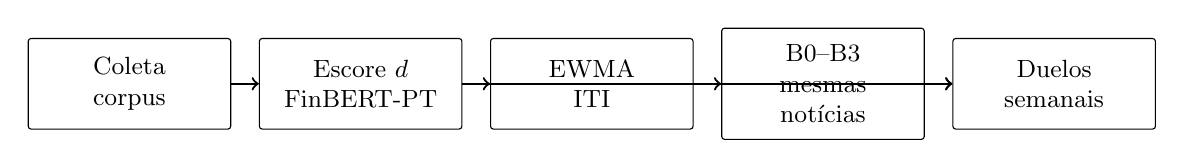
\begin{tikzpicture}[
  font=\small,
  box/.style={draw, rectangle, rounded corners=1pt, align=center, inner sep=6pt, minimum height=1.15cm, text width=2.15cm},
  arr/.style={->, thick}
]
\node[box] (c) {Coleta\\corpus};
\node[box, right=0.35cm of c] (s) {Escore $d$\\FinBERT-PT};
\node[box, right=0.35cm of s] (e) {EWMA\\ITI};
\node[box, right=0.35cm of e] (b) {B0--B3\\mesmas\\notícias};
\node[box, right=0.35cm of b] (r) {Duelos\\semanais};
\draw[arr] (c) -- (s);
\draw[arr] (s) -- (e);
\draw[arr] (s) -- (b);
\draw[arr] (e) -- (r);
\draw[arr] (b) -- (r);
\end{tikzpicture}
\caption{Fluxo operacional: das notícias aos duelos do ITI com alternativas simples.}
\label{fig:pipeline}

\vspace{0.4em}
{\footnotesize Fonte: elaboração própria.}
\end{figure}

Nada neste capítulo afirma que o ITI acrescente informação ao mercado. Afirma só o compromisso de método: coletar com critério, classificar com modelo de domínio, agregar com memória explícita e só então perguntar se o índice diz mais do que contar matérias.

\chapter{Andamentos experimentais}
\label{cap:andamentos}

O que segue não é resultado de dissertação, nem teste de H1. É o registro do que o laboratório \textbf{já executou} e do que isso \textbf{ainda não autoriza} a concluir. O gate de concordância humana no corpus de saneamento \textbf{não foi atingido}; sem ele, associação com retorno permanece exercício de protocolo.

\section{O pipeline roda}

Conseguimos encadear raspagem, corpus tabular, inferência, série do ITI e rotina de comparação semanal. Isso responde a uma pergunta estreita: o desenho do Capítulo~\ref{cap:metodologia} é executável, não só conceitual. Não responde se o índice informa preço.

\section{Classificador no corpus local}

Anotamos cem notícias do recorte Sabesp e comparamos o FinBERT-PT-BR com essa anotação. No artigo de origem, o modelo reporta desempenho bem mais alto em noticiário financeiro amplo \cite{santos2023finbert}. No saneamento, na amostra manual, os números caem abaixo do gate previsto (acurácia da ordem de 70\% ou $\kappa \geq 0{,}40$).

\begin{table}[htbp]
\caption{Concordância do FinBERT-PT-BR com anotação humana no corpus de saneamento (n = 100), ainda exploratória.}
\label{tab:kappa}
\begin{tabular}{|p{0.46\textwidth}|p{0.22\textwidth}|p{0.22\textwidth}|}
\hline
\textbf{Métrica} & \textbf{Valor} & \textbf{Gate} \\
\hline
Acurácia & 48\% & abaixo de 70\% \\
\hline
$\kappa$ de Cohen & 0,163 & abaixo de 0,40 \\
\hline
F1 macro & 0,42 & --- \\
\hline
\end{tabular}

\vspace{0.4em}
{\footnotesize Fonte: elaboração própria a partir da amostra manual do laboratório.}

\end{table}

Dois controles na mesma amostra --- um modelo de tweets em português e um BERT genérico em PT \cite{souza2020bertimbau} --- também ficaram aquém do gate (e, em $\kappa$, piores ou semelhantes). O problema, portanto, não se reduz a ``trocar a arquitetura''. Parte das matérias é \emph{roundup} (agenda de várias empresas no mesmo texto): cerca de um quarto da amostra manual. No subconjunto focal da Sabesp, $\kappa$ sobe um pouco (da ordem de 0,22) e continua abaixo do critério. Contaminação de gênero jornalístico explica parte, não tudo.

Enquanto o gate falhar, o escore $d$ no saneamento é uma ferramenta preliminar. Não tratamos o classificador como validado para o setor.

\section{Campanhas R0 e R1 como exercício de protocolo}

Rodamos o protocolo de vinte e quatro duelos em janelas do caso Sabesp, variando a memória $\alpha$ (por exemplo 0,85 e 0,70) para ver se o pipeline de comparação se comporta de ponta a ponta. Isso é \textbf{ablação operacional}, não estimação definitiva de $\alpha$ e não teste de H1.

Alguns confrontos favorecem o ITI frente a um baseline; a maior parte não. Poucas diferenças passam o bootstrap --- em quantidade compatível com busca múltipla em vinte e quatro testes correlacionados. Sem classificador acima do gate, \textbf{não interpretamos} esses duelos como evidência de que o índice acrescente informação sobre retorno futuro.

O que os exercícios mostram, no máximo, é que o protocolo é reproduzível: mesmas notícias, mesmas métricas, mesmos horizontes, baselines internos, memória explícita. Direção do efeito, magnitude e robustez a outras empresas ficam em aberto, como já alertavam a literatura de reversão \cite{yoshinaga2012sentimento} e a de lags heterogêneos \cite{eramiars2025correlacao}.

\section{O que deliberadamente não fechamos}

Não afirmamos vitória do ITI. Não afirmamos causalidade \cite{utfpr2024bert}. Não promovemos o painel de visualização do laboratório a evidência. Não tratamos Copasa, Sanepar, Granger, volume ou controles de mercado amplo. O Capítulo~\ref{cap:proximos} lista o que ainda falta para a avaliação que a dissertação deverá sustentar perante a banca.

\chapter{Próximos passos}
\label{cap:proximos}

O manuscrito agora cobre fundamentação, desenho operacional e andamentos. Falta a avaliação que possa ser lida como resultado --- e ela depende, primeiro, de um classificador credível no domínio.

Prioridades imediatas:

\begin{enumerate}
  \item Relabel e, se preciso, adaptação do modelo ao gênero jornalístico de saneamento, até o gate de concordância.
  \item Só então reler os duelos ITI versus B0--B3; até lá, H1 permanece hipótese de trabalho.
  \item Estender o corpus a outras empresas listadas de água e esgoto (Copasa, Sanepar), sem misturar o caso âncora com a extensão.
  \item Testes que ainda não rodamos: janelas adicionais, persistência, volume, controles de mercado amplo --- e só se o gate permitir interpretação.
\end{enumerate}

Não encerramos desempenho nem direção do efeito. O compromisso continua o mesmo: coletar com critério, classificar com modelo de domínio, agregar com memória explícita e só então perguntar se o índice acrescenta informação.


\bookmarksetup{startatroot}

\postextual
\bibliographystyle{abntex2-alf}
\bibliography{referencias}

\end{document}
